\chapter{Implementation}
\label{chap:implementation}

In addition to an overview of the simulation environment, the implementation of both the genetic algorithm and the behavior tree will be discussed in this chapter.

\section{Traffic Manager}
A custom-developed Traffic Manger is employed to simulate a traffic environment, which is subsequently controlled by a genetic algorithm. The Traffic Manager is treated as a 'black box' in this master's thesis, with only a brief introduction provided. In essence, it simulates simulate traffic using a start scenario, where the positions and types of actors (vehicles and pedestrians) are defined. Throughout all simulations conducted in this thesis, the Traffic Manager was configured with a frequency of 100Hz and the simulation duration set to 35 seconds.

Each simulation involves at least one EGO vehicle, with the option to include any number of Non-Player Characters (NPCs). The EGO vehicle can be either partly or completely supervised by autonomous driving functions. The goal of the genetic algorithm is to subsequently test these function for requirements like safety and comfort. This is achieved by controlling the NPCs in a way to generate critical scenarios.

\subsection{Action Interface}
\label{sect:implementation:action_interface}
In order to control the behaviour of all actors inside the simulation, actions can be requested via the Action Interface, which is provided by the Traffic Manager. An action initiates a certain behaviour from an actor and can be set at any timestep\footnote{depending on the autonomous driving function under test, the Action Interface might be disabled for the EGO vehicle}. Pedestrians and vehicles have different sets of possible actions. If no action is applied, the actor will behave in a normal manner inside the simulation. This implies that the actor will follow its assigned path until a new action changes its behaviour. It will stick to traffic rules and will break in case of an obstacle. The following list shows all actions which were available for the genetic algorithm at the time of this master's thesis.

\begin{itemize}
	\item JunctionSelection
	\begin{itemize}
		\item vehicle\_id: int, step: int, junction\_selection\_angle (radians): float
		\item Vehicles will choose which direction to take at junctions based the junction\_selection\_angle.
	\end{itemize}
	\item LaneChange
	\begin{itemize}
		\item vehicle\_id: int, step: int, direction: float, distance: float, delay (optional): float
		\item Initiates a lane-change based on its given parameters.
	\end{itemize}
	\item AbortLaneChange
	\begin{itemize}
		\item vehicle\_id: int, step: int
		\item Will abort a current lane-change.
	\end{itemize}
	\item ModifyTargetVelocity
	\begin{itemize}
		\item vehicle\_id: int, step: int, percentage: float
		\item Modifies the internal target velocity of the vehicle by a percentage. If set to 0, the vehicle will stop.
	\end{itemize}
	\item TurnHeading
	\begin{itemize}
		\item pedestrian\_id: int, step: int
		\item The pedestrian will turn 180 degrees and walk in the opposite direction
	\end{itemize}
	\item CrossRoad
	\begin{itemize}
		\item pedestrian\_id: int, step: int
		\item The pedestrian will cross the road immediately.
	\end{itemize}
	\item CrossAtCrosswalk
	\begin{itemize}
		\item pedestrian\_id: int, step: int
		\item The pedestrian will cross the road at the next crosswalk.
	\end{itemize}
\end{itemize}

The genetic algorithm only controls NPCs, while a behaviour tree is used for the EGO vehicle itself. Both methods utilize the Action Interface to guide their respective actors. An overview is provided in Figure \ref{fig:implementation:traffic_manager_structure}.

\begin{figure}[ht] 
	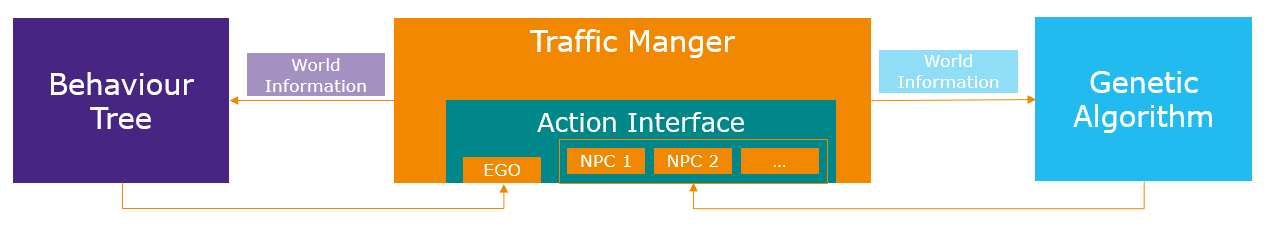
\includegraphics[width=1\linewidth]{figures/tm_structure}
	\caption{Action Interface structure}
	\label{fig:implementation:traffic_manager_structure}
\end{figure}

\section{Genetic Algorithm}
The genetic algorithm will search for sequences of actions that will result in the most interesting scenarios according to its cost function. To implement the genetic algorithm, the Python library DEAP\footnote{\url{https://deap.readthedocs.io/en/master}} was chosen, as it is a popular tool in academia and allows for high customisability. The algorithm has full access to set actions for all NPCs. Searching for sequences of actions, the GA tries to optimize a cost function.

A few default settings for the genetic algorithm were chosen. For example, it was decided, that the genetic algorithm can set an action per actor every 50 steps, which translates to 0.5 seconds (simulation runs at 100hz). In other words, every 50 steps of the simulation is 1 timestep for the genetic algorithm. If the GA decides to not set an action, "NoAction" will be used as a placeholder.

\subsection{Maximum Number of Generations}
A fixed maximum number of generation is a commonly used stopping criteria. While more complex methods like an "adaptive convergence rate" might lead to better performance, it was decided that the additional complexity of having to choose a suitable convergence rate outweighs its potential benefits. Especially considering that a genetic algorithm already has a lot of different control parameters that need tuning. Performance is a big consideration in this thesis, thus a lower maximum number of generations is preferred. During testing, a generation size of 30 was almost always sufficient and will be used in all of the upcoming testing.

\subsection{Encoding}
When implementing a genetic algorithm, it is necessary to use an encoding that fits to the problem at hand. In this context, each chromosome is required to include all actions of one whole simulation. Due to the deterministic nature of the Traffic Manager, it is sufficient to define a simulation by only the action sequence from a chromosome and the initial state, which is defines by a start scenario. The different encodings presented in Section \ref{sect:foundations:chromosomes_and_genes} were not directly applicable to the given problem. Therefore, a custom encoding for both chromosomes and genes needed to be generated.

\subsubsection{Chromosome}
Two different encodings proved to be a good fit. Both use the position of a gene inside the chromosome to define the time step of an action. Which chromosome encoding is the most adequate will be discussed and tested in Chapter \ref{chap:hyperparameter_tuning}.

\paragraph{Time}
The first encoding is called 'Time'. In this encoding, each gene corresponds to 1 time step (1 gene per 0.5 seconds) and needs to contain all actions of all NPCs at that particular moment. A gene is a list with a size equal to the number of NPCs. Each object in this list represents an action. The index of an action inside a gene corresponds to the NPC ID. For example, an action positioned in the gene at index 2, will be applied to NPC 2. If the gene is at position 6 in the chromosome, the action will be set at second 3.0 in the simulation. A visualization is seen in Figure \ref{fig:implementation:encoding_chromosome_time}.

\begin{figure}[ht] 
	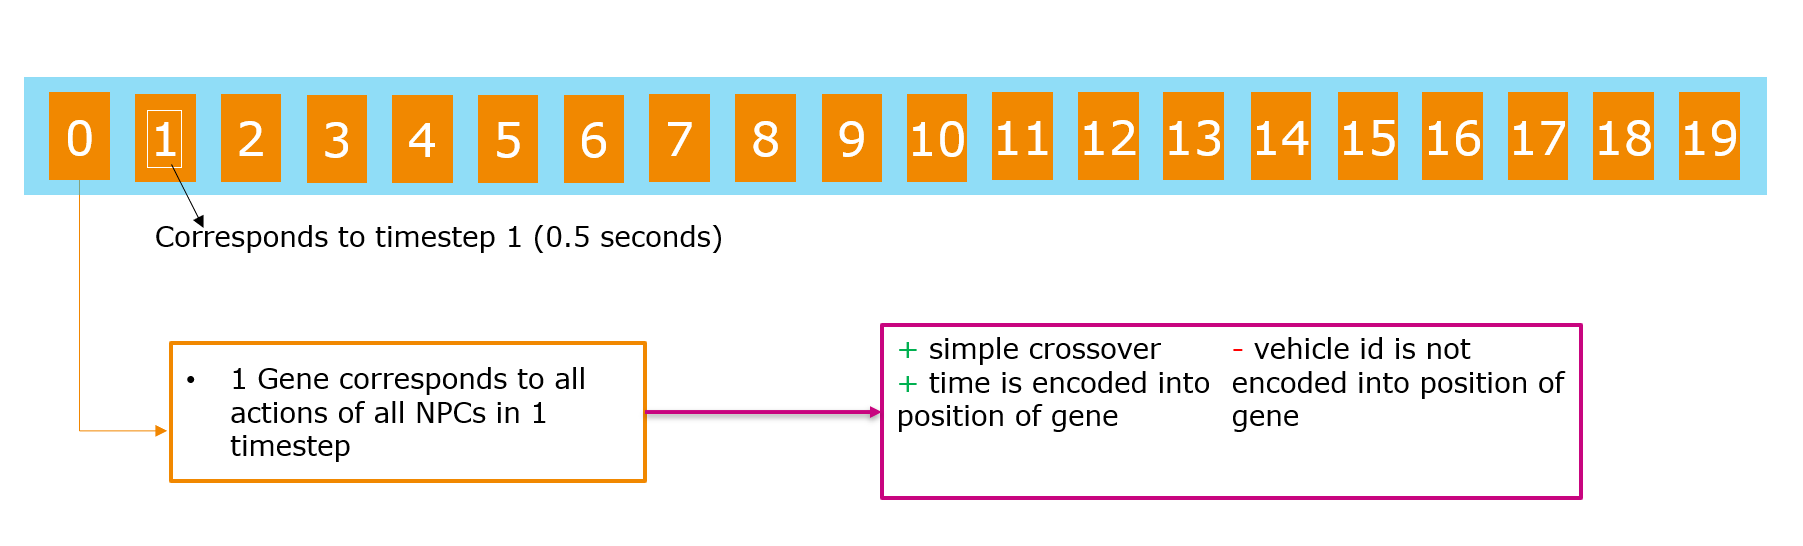
\includegraphics[width=1\linewidth]{figures/time_encoding}
	\caption{Time}
	\label{fig:implementation:encoding_chromosome_time}
\end{figure}

Given the previously stated simulation time of 35 seconds, each chromosome has a length of $35 * 2 = 70$ genes. The crossover operation can only move all actions of a time step at once. Modifications in the timeline between actions of the same time step will only happen through a mutation operation.

\paragraph{Time+NPC}
The second encoding is called 'Time+NPC'. Here, one gene corresponds to exactly one action. In order to not loose required information, the IDs of each NPC must also be encoded into the gene's position in its chromosome. One might visualize this as unfolding the matrix build by the genes and chromosome in the Time encoding into a linear array. Each actor's actions are listed one after another. Now, each gene has a length of $1$ and each chromosome has a length of $35 * 2 * number\_of\_actors$, which makes them much longer compared to the previous encoding. Figure \ref{fig:implementation:encoding_chromosome_time_npc} provides a visualization. In this example, a gene at position 13 corresponds to an action for NPC 2 at time step 3 (which is at 1.5 seconds in the simulation).

\begin{figure}[ht] 
	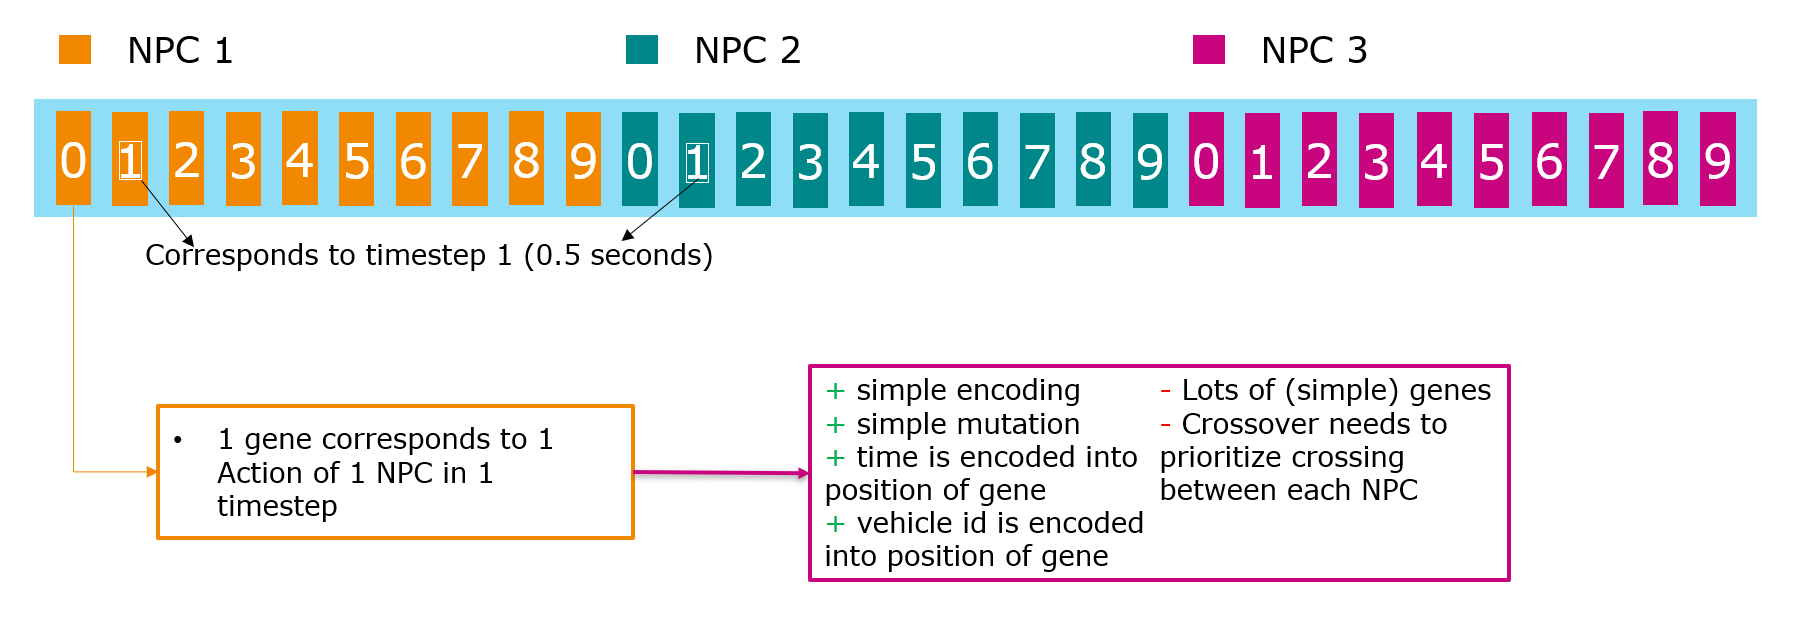
\includegraphics[width=1\linewidth]{figures/time_npc_encoding}
	\caption{Time + NPC}
	\label{fig:implementation:encoding_chromosome_time_npc}
\end{figure}

However for this encoding to make sense, the OnePoint and TwoPoint crossover operations had to be modified in a way, that for each NPC, these crossover operations are applied individually. If this was not the case, OnePoint crossover would introduce changes to actions of only one NPC. Because these different crossover points are chosen independently, the position of the crossing now differs between the NPCs. This modification allows the crossover operation to break up actions at the same time step, which was not possible with the Time encoding.

\subsubsection{Gene}
Two different encodings for genes were implemented. A gene always consists of a list, which depending on the chromosome type either has a length of $number\_of\_actors$ (in case of Time) or of length 1 (in case of Time+NPC). The following two encodings explain the possible objects in these lists. In both encodings, the probability of each action remains the same and can be seen in Table \ref{tab:implementation:action_probabilities}.

\begin{table}[ht]
	\centering
	\begin{tabular}{lc|lc}
		\hline
		\multicolumn{2}{c|}{Vehicles} & \multicolumn{2}{c}{Pedestrians} \\
		ActionType & Probability & ActionType & Probability \\
		\hline
		NoAction & 65\% & NoAction & 84\% \\
		JunctionSelection & 6\% & PedTurnHeading & 2\% \\
		LaneChange & 10\% & PedCrossRoad & 4\% \\
		AbortLaneChange & 2\% & CrossAtCrosswalk & 10\% \\
		ModifyTargetVelocity & 17\% & & \\
		\hline
	\end{tabular}
	\caption{probability of actions}
	\label{tab:implementation:action_probabilities}
\end{table}

These probabilities were manually chosen based on experience. For example, setting PedTurnHeading to a high probability will see many pedestrians change their direction in front of the EGO vehicle multiple times, aiming to initiate emergency breaks by the EGO vehicle. However, this is only critical to a certain extend and the probability is accordingly set to a low value.

\paragraph{Integer}
The first encoding uses integers that are translated into actions when the simulation starts. For each action, a range of integers is assigned; the larger the range, the more likely an action is chosen by the GA. These ranges correspond to the probabilities given in Table \ref{tab:implementation:action_probabilities}.

Actions that have parameters need their assigned integer range to be manually split again. For example, it was decided, that ModifyTargetVelocity has five different percentage settings, namely 50, 70, 100, 130, 160. Therefore, each of these 5 settings needs a unique range of integers assigned, again with different lengths, in order to have different probabilities. A complete list can be seen in Table \ref{tab:implementation:integer_encoding_probabilities}.

\begin{table}[ht]
	\centering
	\begin{tabular}{llc}
		\hline
		ActionType & Parameter & Probability \\
		\hline
		JunctionSelection 	& straight & 34\% \\
		& left & 33\% \\
		& right & 33\% \\
		\hline
		LaneChange 			& left & 50\% \\
		& right & 50\% \\
		\hline
		ModifyTargetVelocity & 50 & 10\%\\
		& 70 & 20\%\\
		& 100 & 45\%\\
		& 130 & 20\%\\
		& 160 & 5\%\\
		\hline
	\end{tabular}
	\caption{Integer encoding: probability of parameters per action}
	\label{tab:implementation:integer_encoding_probabilities}
\end{table}

Combining these ranges results in a continuos list of integers. The genetic algorithm will choose integers in this list for its genes. Before a simulation is started, these integers are then encoded back into actions.

\paragraph{Dictionary}
The second encoding for genes corresponds exactly to the actual actions used in the simulations, requiring no translation. Each action is again selected based on the same probabilities from Table \ref{tab:implementation:action_probabilities}. For actions without parameters, the different encoding will make no difference. However, actions with parameters are no longer split into different discrete settings. Instead, each parameter is chosen by a randomness function, which is individually selected per action. For example in case of the percentage parameter in ModifyTargetVelocity, the values are selected from a gaussian distribution with $mu=100$, $sigma=25$ and a range limit between 0 and 300. An overview is provided in Table \ref{tab:implementation:dict_encoding_probabilities}.
Once again, these probability functions were assigned based on intuition as well as trial and error. 

\begin{table}[ht]
	\centering
	\begin{tabular}{lcc}
		\hline
		ActionType & SelectionFunction & Settings \\
		\hline
		JunctionSelection 	& Choice & [straight, left, right] \\
		LaneChange 			& Choice & [left, right]\\
		ModifyTargetVelocity & Gauss Distribution & Mu: 100, Sigma: 25\\
		\hline
	\end{tabular}
	\caption{Dictionary encoding: probability of parameters per action}
	\label{tab:implementation:dict_encoding_probabilities}
\end{table}

Compared to integer encoding, this method allows for much higher granularity when selecting parameters. However, because only one action type (ModifyTargetVelocity) has a continuos variable, this difference might be insignificant. The contrast between encodings will likely become more pronounced with an increasing number of implemented actions in the Action Interface. Chapter \ref{chap:hyperparameter_tuning} will investigate, if the performance of a genetic algorithm differs between these two encodings.

\subsection{Cost Function}
\label{sect:implementation:cost_function}
This master's thesis utilizes only internal values from the Traffic Manager for the cost function, specifically if the ego vehicle had to initiate an emergency break. As long as the EGO vehicle has no emergency stop initiated, the cost value will increase. If a maximum duration of 3 seconds is exceeded, the cost value will increase as well. Only in cases where none of these two conditions is fulfilled, no cost will be added. This penalty of the maximum duration was introduced to reduce the number of instances, where the ego vehicle is constantly brake-checked\footnote{\enquote{the unsafe action of applying a car’s brakes to dissuade a driver who is following too closely} according to \href{https://www.dictionary.com/e/slang/brake-check/}{https://www.dictionary.com/e/slang/brake-check/}} by the leading vehicle. The cost values are not easily interpreted, so these numbers are modified for this master's thesis using Equation \ref{equ:implementation:modified_cost}.

\begin{equation} 
	\begin{split}
		cummulated\_emergency\_break\_duration & = (3500 - cost) / 100
	\end{split}
	\label{equ:implementation:modified_cost}
\end{equation}

The constant 3500 is used to account for the 100Hz sampling rate and the duration of 35 seconds. The division by 100 transforms the value into seconds. A higher cumulated emergency brake duration is preferable. It is important to consider that this value might not exactly correspond to the actual cumulated emergency brake duration time from the simulation, due to the penalty applied by the cost function for emergency breaks that last longer then 3 seconds.

\section{Behaviour Tree}
The EGO vehicle will be controlled by a behaviour tree, which is implemented using the Python library py\_trees\footnote{\href{https://py-trees.readthedocs.io/en/release-2.2.x/}{https://py-trees.readthedocs.io/en/release-2.2.x/}}. The general idea is to have the EGO vehicle move in a relatable manner trough the world. It will attempt to dodge standing or slow-moving obstacles as well as decide which turn to take at junctions.

\subsection{Structure}
While the behaviour tree has access to the same Action Interface (see Section \ref{sect:implementation:action_interface}) as the genetic algorithm, it needs a higher level of integration with the Traffic Manger. The genetic algorithm is only interested in the resulting emergency break values, but the behaviour tree needs access to internal functions during the simulation. Conditions like NoObstacle() or LaneChangePossible() execute functions from the Traffic Manager to get needed information on the world around the EGO vehicle. Figure \ref{fig:implementation:bt} shows the implemented behaviour tree.

\begin{figure}[ht] 
	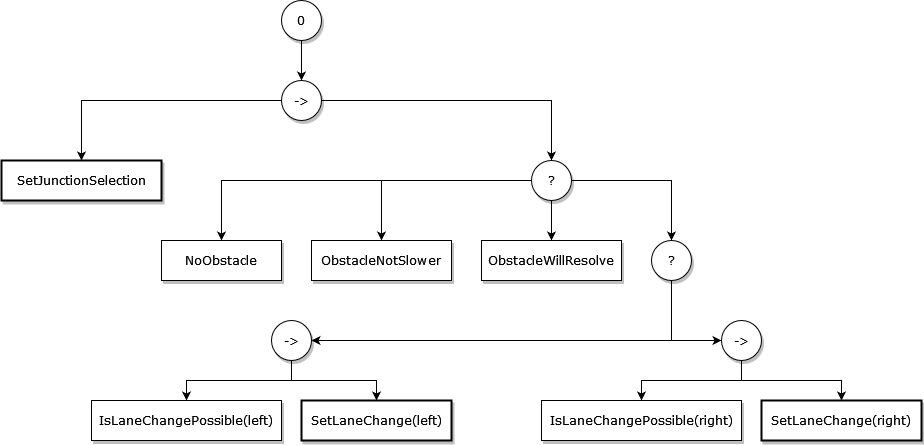
\includegraphics[width=1\linewidth]{figures/behaviorTree}
	\caption{implemented behaviour tree}
	\label{fig:implementation:bt}
\end{figure}

Each tick, the branch junction selection will first get executed, which will switch between the settings "straight", "left" and "right" every 3 seconds. This serves the purpose of generating more interesting situations, as otherwise, the ego vehicle will only move straight. A random junction selection would not be possible, as this would make the simulation non-deterministic. While implementing a navigation system was investigated, it was decided against doing so, as the added complexity did not seem to significantly improve the resulting simulations.

The next branch focuses on dodging obstacles. First, the condition NoObstacle() determines , if an obstacle is on the path of the EGO vehicle. Second, a threshold of 50\% in ObstacleNotSlower() determines if a lane change makes sense. Third, the ObstacleWillResolve() function has the responsibility to check if the obstacle is 1. inside a junction or 2. roughly at a 90 degree angle. In both cases, no takeover will be performed. In case all of the three functions return false, a final function LaneChangePossible() will check, if a lane change to the left is possible and if this is not the case, if a lane change to the right is possible. Depending on its result, a lane change to the suggested direction is performed. LaneChangePossible() might not allow a lane change if 1. there is no lane or 2. if the lane is blocked by an obstacle.


